%% bare_jrnl.tex
%% V1.4b
%% 2015/08/26
%% by Michael Shell
%% see http://www.michaelshell.org/
%% for current contact information.
%%
%% This is a skeleton file demonstrating the use of IEEEtran.cls
%% (requires IEEEtran.cls version 1.8b or later) with an IEEE
%% journal paper.
%%
%% Support sites:
%% http://www.michaelshell.org/tex/ieeetran/
%% http://www.ctan.org/pkg/ieeetran
%% and
%% http://www.ieee.org/

%%*************************************************************************
%% Legal Notice:
%% This code is offered as-is without any warranty either expressed or
%% implied; without even the implied warranty of MERCHANTABILITY or
%% FITNESS FOR A PARTICULAR PURPOSE! 
%% User assumes all risk.
%% In no event shall the IEEE or any contributor to this code be liable for
%% any damages or losses, including, but not limited to, incidental,
%% consequential, or any other damages, resulting from the use or misuse
%% of any information contained here.
%%
%% All comments are the opinions of their respective authors and are not
%% necessarily endorsed by the IEEE.
%%
%% This work is distributed under the LaTeX Project Public License (LPPL)
%% ( http://www.latex-project.org/ ) version 1.3, and may be freely used,
%% distributed and modified. A copy of the LPPL, version 1.3, is included
%% in the base LaTeX documentation of all distributions of LaTeX released
%% 2003/12/01 or later.
%% Retain all contribution notices and credits.
%% ** Modified files should be clearly indicated as such, including  **
%% ** renaming them and changing author support contact information. **
%%*************************************************************************


% *** Authors should verify (and, if needed, correct) their LaTeX system  ***
% *** with the testflow diagnostic prior to trusting their LaTeX platform ***
% *** with production work. The IEEE's font choices and paper sizes can   ***
% *** trigger bugs that do not appear when using other class files.       ***                          ***
% The testflow support page is at:
% http://www.michaelshell.org/tex/testflow/



\documentclass[journal]{IEEEtran}
%
% If IEEEtran.cls has not been installed into the LaTeX system files,
% manually specify the path to it like:
% \documentclass[journal]{../sty/IEEEtran}





% Some very useful LaTeX packages include:
% (uncomment the ones you want to load)


% *** MISC UTILITY PACKAGES ***
%
%\usepackage{ifpdf}
% Heiko Oberdiek's ifpdf.sty is very useful if you need conditional
% compilation based on whether the output is pdf or dvi.
% usage:
% \ifpdf
%   % pdf code
% \else
%   % dvi code
% \fi
% The latest version of ifpdf.sty can be obtained from:
% http://www.ctan.org/pkg/ifpdf
% Also, note that IEEEtran.cls V1.7 and later provides a builtin
% \ifCLASSINFOpdf conditional that works the same way.
% When switching from latex to pdflatex and vice-versa, the compiler may
% have to be run twice to clear warning/error messages.






% *** CITATION PACKAGES ***
%
\usepackage{cite}
% cite.sty was written by Donald Arseneau
% V1.6 and later of IEEEtran pre-defines the format of the cite.sty package
% \cite{} output to follow that of the IEEE. Loading the cite package will
% result in citation numbers being automatically sorted and properly
% "compressed/ranged". e.g., [1], [9], [2], [7], [5], [6] without using
% cite.sty will become [1], [2], [5]--[7], [9] using cite.sty. cite.sty's
% \cite will automatically add leading space, if needed. Use cite.sty's
% noadjust option (cite.sty V3.8 and later) if you want to turn this off
% such as if a citation ever needs to be enclosed in parenthesis.
% cite.sty is already installed on most LaTeX systems. Be sure and use
% version 5.0 (2009-03-20) and later if using hyperref.sty.
% The latest version can be obtained at:
% http://www.ctan.org/pkg/cite
% The documentation is contained in the cite.sty file itself.






% *** GRAPHICS RELATED PACKAGES ***
%
\ifCLASSINFOpdf
 \usepackage[pdftex]{graphicx}
  % declare the path(s) where your graphic files are
  % \graphicspath{{../pdf/}{../jpeg/}}
  % and their extensions so you won't have to specify these with
  % every instance of \includegraphics
 \DeclareGraphicsExtensions{.pdf,.jpeg,.png}
\else
  % or other class option (dvipsone, dvipdf, if not using dvips). graphicx
  % will default to the driver specified in the system graphics.cfg if no
  % driver is specified.
  % \usepackage[dvips]{graphicx}
  % declare the path(s) where your graphic files are
  % \graphicspath{{../eps/}}
  % and their extensions so you won't have to specify these with
  % every instance of \includegraphics
  % \DeclareGraphicsExtensions{.eps}
\fi
% graphicx was written by David Carlisle and Sebastian Rahtz. It is
% required if you want graphics, photos, etc. graphicx.sty is already
% installed on most LaTeX systems. The latest version and documentation
% can be obtained at: 
% http://www.ctan.org/pkg/graphicx
% Another good source of documentation is "Using Imported Graphics in
% LaTeX2e" by Keith Reckdahl which can be found at:
% http://www.ctan.org/pkg/epslatex
%
% latex, and pdflatex in dvi mode, support graphics in encapsulated
% postscript (.eps) format. pdflatex in pdf mode supports graphics
% in .pdf, .jpeg, .png and .mps (metapost) formats. Users should ensure
% that all non-photo figures use a vector format (.eps, .pdf, .mps) and
% not a bitmapped formats (.jpeg, .png). The IEEE frowns on bitmapped formats
% which can result in "jaggedy"/blurry rendering of lines and letters as
% well as large increases in file sizes.
%
% You can find documentation about the pdfTeX application at:
% http://www.tug.org/applications/pdftex





% *** MATH PACKAGES ***
%
%\usepackage{amsmath}
% A popular package from the American Mathematical Society that provides
% many useful and powerful commands for dealing with mathematics.
%
% Note that the amsmath package sets \interdisplaylinepenalty to 10000
% thus preventing page breaks from occurring within multiline equations. Use:
%\interdisplaylinepenalty=2500
% after loading amsmath to restore such page breaks as IEEEtran.cls normally
% does. amsmath.sty is already installed on most LaTeX systems. The latest
% version and documentation can be obtained at:
% http://www.ctan.org/pkg/amsmath





% *** SPECIALIZED LIST PACKAGES ***
%
\usepackage{algorithmic}
% algorithmic.sty was written by Peter Williams and Rogerio Brito.
% This package provides an algorithmic environment fo describing algorithms.
% You can use the algorithmic environment in-text or within a figure
% environment to provide for a floating algorithm. Do NOT use the algorithm
% floating environment provided by algorithm.sty (by the same authors) or
% algorithm2e.sty (by Christophe Fiorio) as the IEEE does not use dedicated
% algorithm float types and packages that provide these will not provide
% correct IEEE style captions. The latest version and documentation of
% algorithmic.sty can be obtained at:
% http://www.ctan.org/pkg/algorithms
% Also of interest may be the (relatively newer and more customizable)
% algorithmicx.sty package by Szasz Janos:
% http://www.ctan.org/pkg/algorithmicx




% *** ALIGNMENT PACKAGES ***
%
%\usepackage{array}
% Frank Mittelbach's and David Carlisle's array.sty patches and improves
% the standard LaTeX2e array and tabular environments to provide better
% appearance and additional user controls. As the default LaTeX2e table
% generation code is lacking to the point of almost being broken with
% respect to the quality of the end results, all users are strongly
% advised to use an enhanced (at the very least that provided by array.sty)
% set of table tools. array.sty is already installed on most systems. The
% latest version and documentation can be obtained at:
% http://www.ctan.org/pkg/array


% IEEEtran contains the IEEEeqnarray family of commands that can be used to
% generate multiline equations as well as matrices, tables, etc., of high
% quality.




% *** SUBFIGURE PACKAGES ***
%\ifCLASSOPTIONcompsoc
%  \usepackage[caption=false,font=normalsize,labelfont=sf,textfont=sf]{subfig}
%\else
%  \usepackage[caption=false,font=footnotesize]{subfig}
%\fi
% subfig.sty, written by Steven Douglas Cochran, is the modern replacement
% for subfigure.sty, the latter of which is no longer maintained and is
% incompatible with some LaTeX packages including fixltx2e. However,
% subfig.sty requires and automatically loads Axel Sommerfeldt's caption.sty
% which will override IEEEtran.cls' handling of captions and this will result
% in non-IEEE style figure/table captions. To prevent this problem, be sure
% and invoke subfig.sty's "caption=false" package option (available since
% subfig.sty version 1.3, 2005/06/28) as this is will preserve IEEEtran.cls
% handling of captions.
% Note that the Computer Society format requires a larger sans serif font
% than the serif footnote size font used in traditional IEEE formatting
% and thus the need to invoke different subfig.sty package options depending
% on whether compsoc mode has been enabled.
%
% The latest version and documentation of subfig.sty can be obtained at:
% http://www.ctan.org/pkg/subfig




% *** FLOAT PACKAGES ***
%
%\usepackage{fixltx2e}
% fixltx2e, the successor to the earlier fix2col.sty, was written by
% Frank Mittelbach and David Carlisle. This package corrects a few problems
% in the LaTeX2e kernel, the most notable of which is that in current
% LaTeX2e releases, the ordering of single and double column floats is not
% guaranteed to be preserved. Thus, an unpatched LaTeX2e can allow a
% single column figure to be placed prior to an earlier double column
% figure.
% Be aware that LaTeX2e kernels dated 2015 and later have fixltx2e.sty's
% corrections already built into the system in which case a warning will
% be issued if an attempt is made to load fixltx2e.sty as it is no longer
% needed.
% The latest version and documentation can be found at:
% http://www.ctan.org/pkg/fixltx2e


%\usepackage{stfloats}
% stfloats.sty was written by Sigitas Tolusis. This package gives LaTeX2e
% the ability to do double column floats at the bottom of the page as well
% as the top. (e.g., "\begin{figure*}[!b]" is not normally possible in
% LaTeX2e). It also provides a command:
%\fnbelowfloat
% to enable the placement of footnotes below bottom floats (the standard
% LaTeX2e kernel puts them above bottom floats). This is an invasive package
% which rewrites many portions of the LaTeX2e float routines. It may not work
% with other packages that modify the LaTeX2e float routines. The latest
% version and documentation can be obtained at:
% http://www.ctan.org/pkg/stfloats
% Do not use the stfloats baselinefloat ability as the IEEE does not allow
% \baselineskip to stretch. Authors submitting work to the IEEE should note
% that the IEEE rarely uses double column equations and that authors should try
% to avoid such use. Do not be tempted to use the cuted.sty or midfloat.sty
% packages (also by Sigitas Tolusis) as the IEEE does not format its papers in
% such ways.
% Do not attempt to use stfloats with fixltx2e as they are incompatible.
% Instead, use Morten Hogholm'a dblfloatfix which combines the features
% of both fixltx2e and stfloats:
%
% \usepackage{dblfloatfix}
% The latest version can be found at:
% http://www.ctan.org/pkg/dblfloatfix




%\ifCLASSOPTIONcaptionsoff
%  \usepackage[nomarkers]{endfloat}
% \let\MYoriglatexcaption\caption
% \renewcommand{\caption}[2][\relax]{\MYoriglatexcaption[#2]{#2}}
%\fi
% endfloat.sty was written by James Darrell McCauley, Jeff Goldberg and 
% Axel Sommerfeldt. This package may be useful when used in conjunction with 
% IEEEtran.cls'  captionsoff option. Some IEEE journals/societies require that
% submissions have lists of figures/tables at the end of the paper and that
% figures/tables without any captions are placed on a page by themselves at
% the end of the document. If needed, the draftcls IEEEtran class option or
% \CLASSINPUTbaselinestretch interface can be used to increase the line
% spacing as well. Be sure and use the nomarkers option of endfloat to
% prevent endfloat from "marking" where the figures would have been placed
% in the text. The two hack lines of code above are a slight modification of
% that suggested by in the endfloat docs (section 8.4.1) to ensure that
% the full captions always appear in the list of figures/tables - even if
% the user used the short optional argument of \caption[]{}.
% IEEE papers do not typically make use of \caption[]'s optional argument,
% so this should not be an issue. A similar trick can be used to disable
% captions of packages such as subfig.sty that lack options to turn off
% the subcaptions:
% For subfig.sty:
% \let\MYorigsubfloat\subfloat
% \renewcommand{\subfloat}[2][\relax]{\MYorigsubfloat[]{#2}}
% However, the above trick will not work if both optional arguments of
% the \subfloat command are used. Furthermore, there needs to be a
% description of each subfigure *somewhere* and endfloat does not add
% subfigure captions to its list of figures. Thus, the best approach is to
% avoid the use of subfigure captions (many IEEE journals avoid them anyway)
% and instead reference/explain all the subfigures within the main caption.
% The latest version of endfloat.sty and its documentation can obtained at:
% http://www.ctan.org/pkg/endfloat
%
% The IEEEtran \ifCLASSOPTIONcaptionsoff conditional can also be used
% later in the document, say, to conditionally put the References on a 
% page by themselves.




% *** PDF, URL AND HYPERLINK PACKAGES ***
%
%\usepackage{url}
% url.sty was written by Donald Arseneau. It provides better support for
% handling and breaking URLs. url.sty is already installed on most LaTeX
% systems. The latest version and documentation can be obtained at:
% http://www.ctan.org/pkg/url
% Basically, \url{my_url_here}.




% *** Do not adjust lengths that control margins, column widths, etc. ***
% *** Do not use packages that alter fonts (such as pslatex).         ***
% There should be no need to do such things with IEEEtran.cls V1.6 and later.
% (Unless specifically asked to do so by the journal or conference you plan
% to submit to, of course. )


% correct bad hyphenation here
\hyphenation{op-tical net-works semi-conduc-tor}


\begin{document}
%
% paper title
% Titles are generally capitalized except for words such as a, an, and, as,
% at, but, by, for, in, nor, of, on, or, the, to and up, which are usually
% not capitalized unless they are the first or last word of the title.
% Linebreaks \\ can be used within to get better formatting as desired.
% Do not put math or special symbols in the title.
\title{Combining microstepping and modelling to achieve precision in fossil photogrammetry}
%
%
% author names and IEEE memberships
% note positions of commas and nonbreaking spaces ( ~ ) LaTeX will not break
% a structure at a ~ so this keeps an author's name from being broken across
% two lines.
% use \thanks{} to gain access to the first footnote area
% a separate \thanks must be used for each paragraph as LaTeX2e's \thanks
% was not built to handle multiple paragraphs
%

\author{Alysson Fernandes Mazoni,
        Carolina Zabini,
        and Joao Mauricio Rosario% <-this % stops a space
\thanks{A. F. Mazoni and J. M. Rosario are with the Faculty
of Mechanical Engineering, University of Campinas, Campinas,
Sao Paulo, Brazil.}% <-this % stops a space
\thanks{Carolina Zabini is with the Institute of Geosciences, University of Campinas, Campinas,
Sao Paulo, Brazil.}}

% note the % following the last \IEEEmembership and also \thanks - 
% these prevent an unwanted space from occurring between the last author name
% and the end of the author line. i.e., if you had this:
% 
% \author{....lastname \thanks{...} \thanks{...} }
%                     ^------------^------------^----Do not want these spaces!
%
% a space would be appended to the last name and could cause every name on that
% line to be shifted left slightly. This is one of those "LaTeX things". For
% instance, "\textbf{A} \textbf{B}" will typeset as "A B" not "AB". To get
% "AB" then you have to do: "\textbf{A}\textbf{B}"
% \thanks is no different in this regard, so shield the last } of each \thanks
% that ends a line with a % and do not let a space in before the next \thanks.
% Spaces after \IEEEmembership other than the last one are OK (and needed) as
% you are supposed to have spaces between the names. For what it is worth,
% this is a minor point as most people would not even notice if the said evil
% space somehow managed to creep in.



% The paper headers
\markboth{Journal of \LaTeX\ Class Files,~Vol.~X, No.~Y, June~2020}%
{Shell \MakeLowercase{\textit{et al.}}: Bare Demo of IEEEtran.cls for IEEE Journals}
% The only time the second header will appear is for the odd numbered pages
% after the title page when using the twoside option.
% 
% *** Note that you probably will NOT want to include the author's ***
% *** name in the headers of peer review papers.                   ***
% You can use \ifCLASSOPTIONpeerreview for conditional compilation here if
% you desire.




% If you want to put a publisher's ID mark on the page you can do it like
% this:
%\IEEEpubid{0000--0000/00\$00.00~\copyright~2015 IEEE}
% Remember, if you use this you must call \IEEEpubidadjcol in the second
% column for its text to clear the IEEEpubid mark.



% use for special paper notices
%\IEEEspecialpapernotice{(Invited Paper)}




% make the title area
\maketitle

% As a general rule, do not put math, special symbols or citations
% in the abstract or keywords.
\begin{abstract}
There are several low cost designs for three-dimensional microscope applied to a wide range of applications. Microscopes of this kind are particularly useful in paleontology and biology research projects. The study of small scale fossils benefits greatly from theses devices. In this work, we propose a technique that improves on the precision of these devices using mathematical modelling, feedback control and microstepping of motors. In our approach we can achieve precision by one order of magnitude better than usually applied thanks to the microstepping technique.
\end{abstract}

% Note that keywords are not normally used for peerreview papers.
\begin{IEEEkeywords}
Photogrammetry, 3d imaging, fossil imaging, feedback control.
\end{IEEEkeywords}


% For peer review papers, you can put extra information on the cover
% page as needed:
% \ifCLASSOPTIONpeerreview
% \begin{center} \bfseries EDICS Category: 3-BBND \end{center}
% \fi
%
% For peerreview papers, this IEEEtran command inserts a page break and
% creates the second title. It will be ignored for other modes.
\IEEEpeerreviewmaketitle



\section{Introduction}
% The very first letter is a 2 line initial drop letter followed
% by the rest of the first word in caps.
% 
% form to use if the first word consists of a single letter:
% \IEEEPARstart{A}{demo} file is ....
% 
% form to use if you need the single drop letter followed by
% normal text (unknown if ever used by the IEEE):
% \IEEEPARstart{A}{}demo file is ....
% 
% Some journals put the first two words in caps:
% \IEEEPARstart{T}{his demo} file is ....
% 
% Here we have the typical use of a "T" for an initial drop letter
% and "HIS" in caps to complete the first word.
\IEEEPARstart{T}{he} study of fossils in paleontology have recently gained the aid of three-dimensional models. Typical characteristics of species can be measured as morphometry of fossils and the information obtained can provide data to discuss on the species and their paleoecology, \cite{Mallison2014}. This is particularly true in the context of the discipline of taphonomy, taxonomic studies, where data can provide morphological aspects that help to identify past diversities. Also, taphonomic studies can benefit from this technique, once information can be collectively taken from paviments with several specimens in order to reach interpretations on past ecological dynamics, \cite{Falkingham2012}.

Several papers have already discussed 3D modeling on fossils (\cite{Sutton2001,Caracuel2002,Falkingham2012,Falkingham2013,Hamm2018,Valverde-bastidas2020}) or even on outcrops (\cite{Caracuel2000,Cruzado-caballero2019}). Each technique usually depends on the type of preservation (if the matrix is differentiated from the fossil itself), size of the fossil specimen, and the need for high image resolution. Here, we present a technique developed for the acquisition of morphometric information and superficial ornamentation of small sized macrofossils. The most valuable information developed here is the high resolution obtained from a simple DIY device (which can be printed in a 3D printer) and independence of expensive softwares to provide the final image; everything can be done printing the parts of the microscope, acquiring some commercial components such as the camera, cables, LEDs, motor and driver, microcontroller and manage the lights, positioning and capturing the pictures using an Arduino and a computer program in Python. 


% You must have at least 2 lines in the paragraph with the drop letter
% (should never be an issue)

There are several types of three dimensional microscopes and other equipment aimed at generating models that can obtain such information. In most cases, they rely on laser or structured lighting and are very precise and expensive devices, \cite{Remondino2012,Rawat2017}.


\subsection{Photogrammetry based three-dimensional microscopes}

In many cases in paleontology, small scale fossils are of interest. The small scale fossils here mentioned range from a milimeter to a few centimeters. In theses cases, photogrammetry techniques are available. They need simple digital cameras or handheld microscope and programs or software packages able to process theses images. 

In these programs, two main techniques are used, one of them is by pointing different light sources to the object studied and a surface is estimated using patterns of light and shade in several images taken in every light condition. This technique is dependent on the surface of the material: there must not be too much reflections of light, \cite{Queau2015,Saracchini2013}.

Another technique is taking images with the same orientation but at different distances from the object studied. Each image will possess a separate focal region in the object. So, a cloud of points can be taken as the different heights from the focal point, \cite{Saracchini2012,Saracchini2011}.

Devices using both principles can be built in low cost designs and a combination of the two techniques is also possible, \cite{Wijnen2016,Schneidereit2017,Lelis2017,Schaefer2012,Cavas-martinez2019,Campbell2014}. The precision achieved with the first method is increased by using several light sources from different directions as well as using punctual sources so as to have very distinct ray dispersion patterns. On the second method the precision is grossly limited by the step size taken from one picture to another. This is the case since the step must be known.

The processes used in this last technique can be carried out manually using a positioning device such as the ones used in scanning electron microscope along the a digital camera or simple portable microscope. The processes is easily automatized with a positioning system operated by a stepping motor and a gear mechanism that allows to know beforehand the distance variation after every step in the motor. This assembly is the standard used in many commercial products.

Stepping motors are a common tool for automation since their can be put to precise positions without a measuring device, such as an encoder. Recently, with the availability of power driver circuits they can be made to operate at fractions as small as $\frac{1}{64}$ of one step. Nominally, this operation can improve precision in positioning applications by two orders of magnitude. This mode of operation is called microstepping, \cite{Kim2013,Kim2013a,Chen2010,Baluta2007}.

In practice, the microstepping operation only guarantees position in fraction of the nominal torque, reduction its practical application to situations to ensure smooth transitions of whole steps, reducing vibrations. This approach eases techniques applied for position control, \cite{Bellini2007,Li2009,Defoort2009,Bendjedia2012,Chen2010}.

In this work, it is proposed a methodology that will take into account the microstepping ability of power driver circuits to improve precision by using a second order linear model to be identified and using as a predictor or the true position of the positioning system. This is also achieved with by adding and encoder and a spring to the system.


% needed in second column of first page if using \IEEEpubid
%\IEEEpubidadjcol


% An example of a floating figure using the graphicx package.
% Note that \label must occur AFTER (or within) \caption.
% For figures, \caption should occur after the \includegraphics.
% Note that IEEEtran v1.7 and later has special internal code that
% is designed to preserve the operation of \label within \caption
% even when the captionsoff option is in effect. However, because
% of issues like this, it may be the safest practice to put all your
% \label just after \caption rather than within \caption{}.
%
% Reminder: the "draftcls" or "draftclsnofoot", not "draft", class
% option should be used if it is desired that the figures are to be
% displayed while in draft mode.
%
%\begin{figure}[!t]
%\centering
%\includegraphics[width=2.5in]{myfigure}
% where an .eps filename suffix will be assumed under latex, 
% and a .pdf suffix will be assumed for pdflatex; or what has been declared
% via \DeclareGraphicsExtensions.
%\caption{Simulation results for the network.}
%\label{fig_sim}
%\end{figure}

% Note that the IEEE typically puts floats only at the top, even when this
% results in a large percentage of a column being occupied by floats.


% An example of a double column floating figure using two subfigures.
% (The subfig.sty package must be loaded for this to work.)
% The subfigure \label commands are set within each subfloat command,
% and the \label for the overall figure must come after \caption.
% \hfil is used as a separator to get equal spacing.
% Watch out that the combined width of all the subfigures on a 
% line do not exceed the text width or a line break will occur.
%
%\begin{figure*}[!t]
%\centering
%\subfloat[Case I]{\includegraphics[width=2.5in]{box}%
%\label{fig_first_case}}
%\hfil
%\subfloat[Case II]{\includegraphics[width=2.5in]{box}%
%\label{fig_second_case}}
%\caption{Simulation results for the network.}
%\label{fig_sim}
%\end{figure*}
%
% Note that often IEEE papers with subfigures do not employ subfigure
% captions (using the optional argument to \subfloat[]), but instead will
% reference/describe all of them (a), (b), etc., within the main caption.
% Be aware that for subfig.sty to generate the (a), (b), etc., subfigure
% labels, the optional argument to \subfloat must be present. If a
% subcaption is not desired, just leave its contents blank,
% e.g., \subfloat[].


% An example of a floating table. Note that, for IEEE style tables, the
% \caption command should come BEFORE the table and, given that table
% captions serve much like titles, are usually capitalized except for words
% such as a, an, and, as, at, but, by, for, in, nor, of, on, or, the, to
% and up, which are usually not capitalized unless they are the first or
% last word of the caption. Table text will default to \footnotesize as
% the IEEE normally uses this smaller font for tables.
% The \label must come after \caption as always.
%
%\begin{table}[!t]
%% increase table row spacing, adjust to taste
%\renewcommand{\arraystretch}{1.3}
% if using array.sty, it might be a good idea to tweak the value of
% \extrarowheight as needed to properly center the text within the cells
%\caption{An Example of a Table}
%\label{table_example}
%\centering
%% Some packages, such as MDW tools, offer better commands for making tables
%% than the plain LaTeX2e tabular which is used here.
%\begin{tabular}{|c||c|}
%\hline
%One & Two\\
%\hline
%Three & Four\\
%\hline
%\end{tabular}
%\end{table}


% Note that the IEEE does not put floats in the very first column
% - or typically anywhere on the first page for that matter. Also,
% in-text middle ("here") positioning is typically not used, but it
% is allowed and encouraged for Computer Society conferences (but
% not Computer Society journals). Most IEEE journals/conferences use
% top floats exclusively. 
% Note that, LaTeX2e, unlike IEEE journals/conferences, places
% footnotes above bottom floats. This can be corrected via the
% \fnbelowfloat command of the stfloats package.

\section{Methodology}

Three dimensional microscopes assembled with a stepper motor as a positioning device are limited to be as precise as the distance increased by one step in their mechanical design. Also, the axis the motor operates must be rigidly coupled with its own axis so as to avoid lost of steps in the process. This also risks vibration given the presence of a relatively large inertia of the mechanical system and camera taken concurrently to move.

The presence of a linear spring between motor and positioning axis can work as an damper to vibrations of this type. However, it will introduce a natural oscillation at a much lower frequency. The idea presented here is to work precisely with the model for this oscillation allowing the operation of the motor compensate the spring`s deflection, achieve precision smaller that one step, using microstepping and simultaneously controlling vibration.

The calibration of such a system to be used generating three dimensional models can be made using a ruler whose image is registered in many positions of operating range. The variation in the size of the ruler inside the image can be used to measure the step with standard precision given the dimensions of the ruler.

\subsection{Microstepping and measuring}

Given a stepper motor that can be placed in a particular reference angle using microsteps and a mechanical system coupled to it, one can suppose that the microsteps are correctly performed by the motor and the angle of the whole system can be measured using an encoder at the other end. Between the motor axis and the screw that moves the microscope and its support part there is a flexible coupling, working as a spring.

In an assembly such as this, the difference from motor angle and system angle is intermediated by a linear inertia-spring system. The spring will take variations in the microsteps and pass them to the other rigid part.

The other rigid part has its rotation measured by an encoder, which can only take half steps as readings. In this point, a model is useful to have measurements interpolated from inputs of microsteps and an encoder steps.

\subsection{Inertia-spring linear system}

Given a stepper motor that can be placed in a particular reference angle $\theta_r$ and an encoder that reads the system rotation as $\theta$, one can assume the presence of a rotation inertia ($J$), a linear stiffness ($k$) for the spring, and a damping to account for friction in both axes ($c$ and $b$). 

In Newton`s Second Law,
\begin{equation}
    J\ddot{\theta} = k(\theta_r-\theta)-c(\dot{\theta}-\dot{\theta}_r)-b\dot{\theta}
\end{equation}
and taking $\theta$ as the output and $\theta_r$ as the input,
\begin{equation}
        J\ddot{\theta} + (c+b)\dot{\theta}+k\theta=c\dot{\theta}_r+k\theta_r
\end{equation}

A Laplace transform can be used to represent a linear model
\begin{equation}
    \frac{\theta(s)}{\theta_r(s)} = \frac{cs+k}{Js^2+(c+b)s+k}
    \label{eq:model}
\end{equation}
the solution of the model in time (convolution) is an estimator for the angle $\theta$ given the input $\theta_r$ and $\dot{\theta}_r$ estimated in the trajectory generated for the motor.


The angle in the encoder is to be converted to a distance once the screw step is known. In order to find the parameters of the model in equation \ref{eq:model}, the system identification theory is appropriate. The stepper motor is moved to oscillation in sinusoidal fashion using the microsteps of input as $\theta_r$ and the frequency of the oscillations is slowly increased with the correspondent response in $\theta$ being measured. 

In the theory of estimation for impulse response, the transfer function of equation \ref{eq:model} can be found using the technique of eigensystems realization using the two signals described ($\theta_r$ applied and $\theta$ measured), \cite{Ljung1999}.

\subsection{Image calibration}

Another way to obtain parameters to feed the identification algorithm is to evaluate the change in distance using a ruler with known dimensions as previously stated. The ratio between the dimensions of the ruler and its appearance on captured images can be used to obtain a distance from a triangle rule. Again, the values thus obtained can be used as data to an identification algorithm. The precision in the case can be evaluated in intermediary steps of the encoder measurement.


\section{Implementation}

The design is inspired on a previous project (described in \cite{Lelis2017}) with the new elements included, namely spring and encoder. Some parts are 3d printed and others are commercially available mechanical components, which amounts to better precision and availability.

\subsection{Mechanical system and electronics}

Models for the printed parts are available as well as specification for the commercial parts. The use of only commercial parts in the main axis of the equipment, from stepper motor renders the design more precise than the original design. This way, the printed parts are made in resin and the ready-made parts are metallic. Figure \ref{fig:picture} shows a picture of the prototype built.

\begin{figure}[!t]
\centering
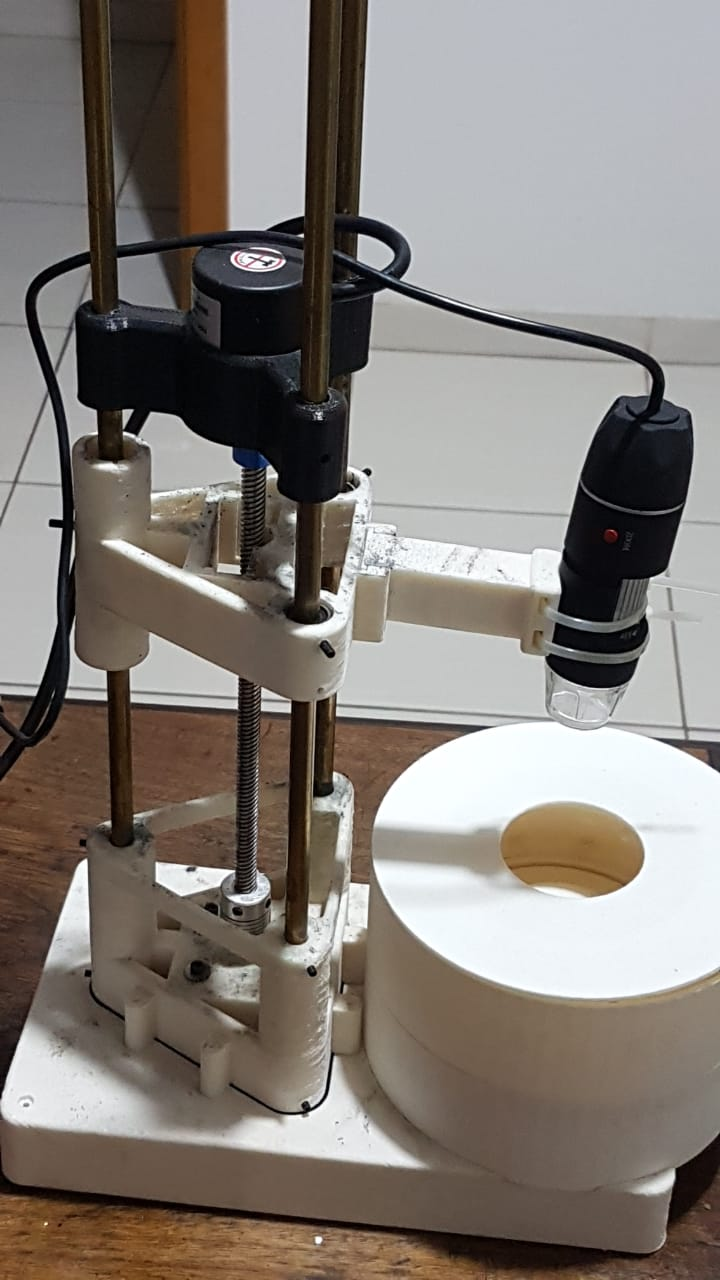
\includegraphics[width=2.5in]{microscope.jpeg}
\caption{Prototype for the system.}
\label{fig:picture}
\end{figure}

The stepper motor is operated by the power circuit A4988 manufactured by Pololu that has become commonplace in 3d printers and many research prototypes, \cite{A4988}. It operates a stepper motor NEMA 17. The control is programmed in a Arduino One that communicates to a computer with a handheld microscope with a possible 800 times magnification. A Python program operates the microscope taking pictures and dispatching positioning signals that make the trajectory to be followed. It sets the distance so the microsteps are taking compensating with the model until the position is achieved.

\subsection{Programs}

A diagram for signals is shown in figure \ref{fig:diagram}. There, a computer operates a microscope or high definition digital camera in order to capture pictures that will be used, alongside with the precise positions in which they were took. Using these images, a function is used according to the technique described in the literature to determine the focal distance that changes in every picture. When the region of the image perfectly focused is reached, its height is determined. Since the process is repeated in many positions, a map of points can be assembled as height levels just as precise as the steps taken. This calculation can be performed after all images are taken.

\begin{figure}[!t]
\centering
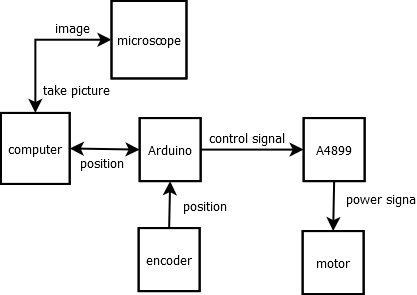
\includegraphics[width=2.5in]{microscope.png}
\caption{Diagram for signals in the microscope design.}
\label{fig:diagram}
\end{figure}

The program sends a message when the picture is taken to the Arduino. In the Arduino's memory, the program start generating microsteps and estimates the current position of the axis angle using a discretized form of equation \ref{eq:model}. This model is an observer for a PI control technique that adjusts the microsteps until the next position is achieved. In this point, this program sends a message to the Python program allowing it to take another picture.

Using the set of pictures taken with positions determined, the same procedure described in recent projects can be used to estimate a mesh of 3D points, in this case with improved precision given better slicing of the images with focal point variation.


\section{Results}

\subsection{Model identification}

In order to estimate the parameters of the observer model, the motor is subjected to turn in a sinusoidal reference with frequencies ranging from 0.001 to 10 Hz. The variation is linear and lasting 1000~s.

This application of this signal to the actuator generates a response shown if figure \ref{fig:chirp_response}. The response signal is input to an impulse response estimation algorithm and eigensystem realization algorithm, \cite{Ljung1999}. The identification process results in the parameters in table \ref{tab:model_parameters}.

\begin{table}[!t]
%% increase table row spacing, adjust to taste
\renewcommand{\arraystretch}{1.3}
% if using array.sty, it might be a good idea to tweak the value of
% \extrarowheight as needed to properly center the text within the cells
\caption{Parameters for the second order model for the system.}
\label{tab:model_parameters}
\centering
%% Some packages, such as MDW tools, offer better commands for making tables
%% than the plain LaTeX2e tabular which is used here.
\begin{tabular}{|c||c|}
\hline
Parameter & Value\\
\hline
inertia ($J$) & 2.43E-3 \\
stiffness ($k$) & 5.21 \\
position damping ($c$) & 1.23E-2 \\
motor damping ($b$) & 7.67E-3\\
\hline
\end{tabular}
\end{table}

\begin{figure}[!t]
\centering
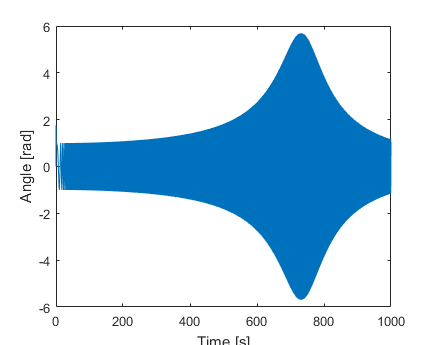
\includegraphics[width=3.5in]{chirp_response.png}
\caption{Response to varying frequency sine.}
\label{fig:chirp_response}
\end{figure}


\begin{figure}[!t]
\centering
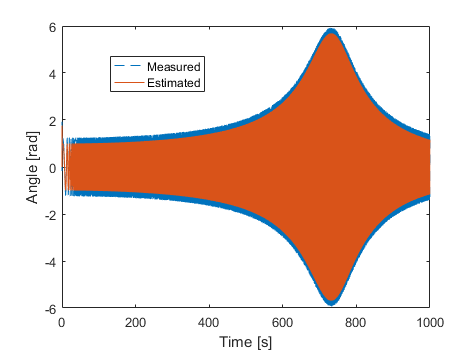
\includegraphics[width=3.5in]{chirp_response_real.png}
\caption{Response to varying frequency sine real and estimated.}
\label{fig:chirp_response_estimated}
\end{figure}



The same signal can be applied again to the system in order to test for its accuracy, comparing reference signal and estimated signal in time in figure \ref{fig:chirp_response_estimated} we can see the dynamical behavior of the observer when applied to the real system.

\subsection{Control tests}

\begin{figure}[!t]
\centering
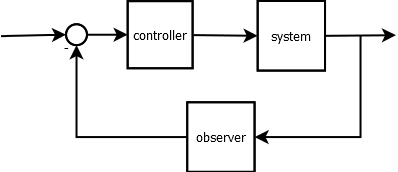
\includegraphics[width=3.5in]{control_loop.png}
\caption{Control loop for the positioning system.}
\label{fig:control_loop}
\end{figure}

Since an observer is obtained by identification, it is intended to used in a PI control scheme as illustrated in figure ??. The control parameters are calculated in a frequency response graphical inspection in the Nyquist diagram in figure \ref{fig:nyquist}. Using parameters $20$ and $1$ respectively in proportional and integral gain results in a complete control system. Its test against the same reference signal is presented in figure \ref{fig:controlled_chirp_response}.

\begin{figure}[!t]
\centering
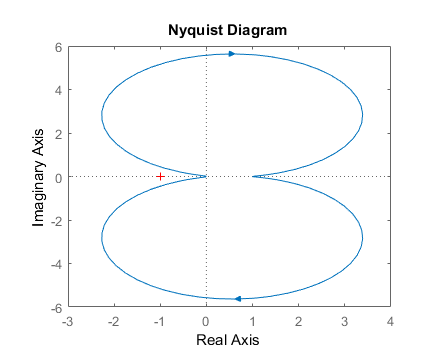
\includegraphics[width=3.5in]{nyquist_microscope.png}
\caption{Nyquist plot for the identified transfer function.}
\label{fig:nyquist}
\end{figure}

\begin{figure}[!t]
\centering
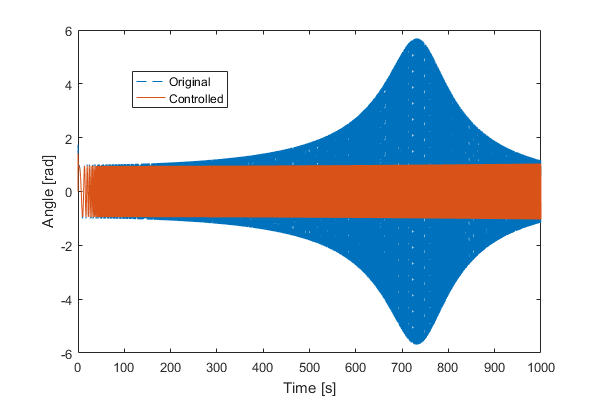
\includegraphics[width=3.5in]{controlled_chirp_response.png}
\caption{Response to varying frequency sine with control.}
\label{fig:controlled_chirp_response}
\end{figure}

\begin{figure}[!t]
\centering
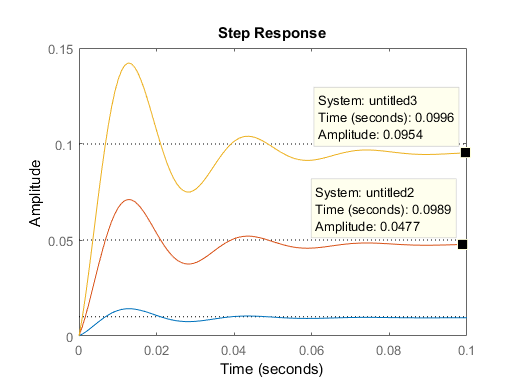
\includegraphics[width=3.5in]{step_response.png}
\caption{Step responses with control.}
\label{fig:step_response}
\end{figure}

Figure \ref{fig:step_response} shows the step responses of the controlled system. We can see that a stationary error of 0.0023 rad for a step with 0.5 rad amplitude and 0.0046 rad for a 0.1 rad step. It represents a 4.6\% stationary error. When considering the original possibility of using precision given by full steps, the control technique used with modelling can improve precision up to 21 times.

\subsection{Example fossil}

With the system already in place, it can capture a set of a 100 images of a fossil and their positions used to assemble a 3D surface map using the algorithm of photogrammetry using variation of focal distance.

The codes are publicly available at a Git repository and can be used in a similar design. The fossil used as example and its mesh are in figures \ref{fig:fossil} and \ref{fig:fossil_3d}.    

\begin{figure}[!t]
\centering
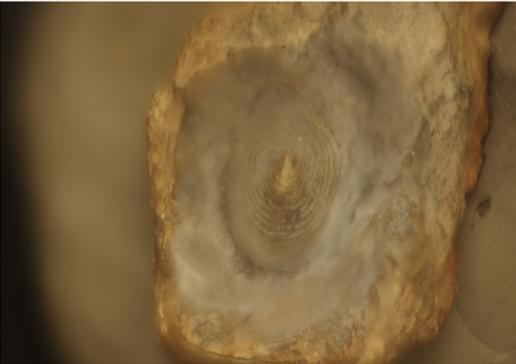
\includegraphics[width=3.5in]{fossil.png}
\caption{Example fossil.}
\label{fig:fossil}
\end{figure}

\begin{figure}[!t]
\centering
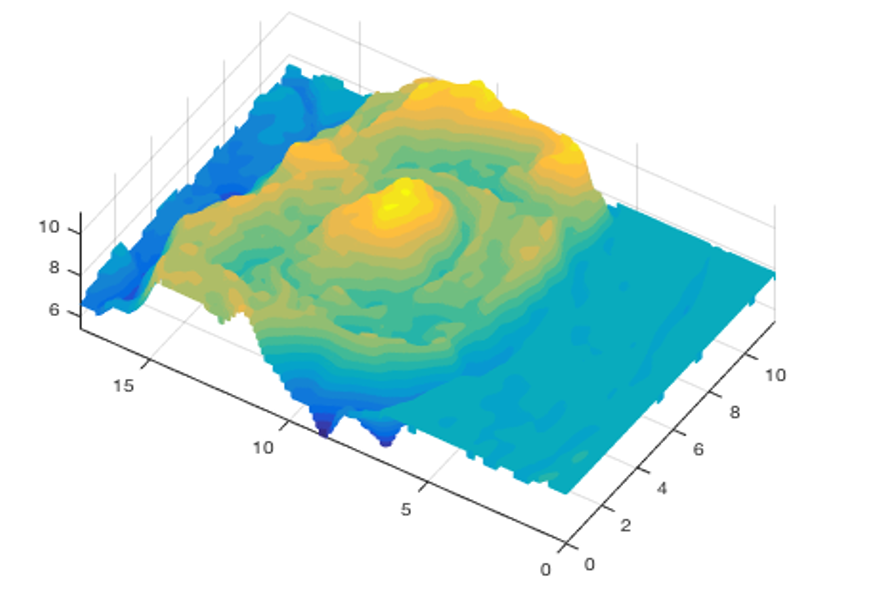
\includegraphics[width=3.5in]{fossil_3d.png}
\caption{Three-dimensional mesh.}
\label{fig:fossil_3d}
\end{figure}


\section{Conclusion}

The use of system modelling is common practice in design problems but are rarely used in its full extent during operation of position control systems. The widespread use of stepping motors creates the possibility for improved precision using the microstepping available in commercial drivers. The imprecision originated from vibration and elasticity are compensated using a mathematical modelling and a feedback control loop with an encoder. This particular design allows a precision improved by 21 times.

The design is limited by the precision of the encoder, stepping motor and driver circuit. Other limitations yet to be studied are the range of sizes that can be operated with this technique, since a position by a range of more than a few tenths of centimeters can involve low frequency or stationary deflection of the whole device.

It is also to be investigated the combination of images here generated with the technique of directional light for the final step of mesh generation.


% if have a single appendix:
%\appendix[Proof of the Zonklar Equations]
% or
%\appendix  % for no appendix heading
% do not use \section anymore after \appendix, only \section*
% is possibly needed

% use appendices with more than one appendix
% then use \section to start each appendix
% you must declare a \section before using any
% \subsection or using \label (\appendices by itself
% starts a section numbered zero.)
%


%\appendices
%\section{Control program}
%Appendix one text goes here.

% you can choose not to have a title for an appendix
% if you want by leaving the argument blank
%\section{Positioning control program}
%Appendix two text goes here.


% use section* for acknowledgment
\section*{Acknowledgment}


The authors would like to thank Fapesp (2017/10956-5) for the financial support and CTI - Renato Archer for help with printing model parts.

% Can use something like this to put references on a page
% by themselves when using endfloat and the captionsoff option.
\ifCLASSOPTIONcaptionsoff
  \newpage
\fi



% trigger a \newpage just before the given reference
% number - used to balance the columns on the last page
% adjust value as needed - may need to be readjusted if
% the document is modified later
%\IEEEtriggeratref{8}
% The "triggered" command can be changed if desired:
%\IEEEtriggercmd{\enlargethispage{-5in}}

% references section

% can use a bibliography generated by BibTeX as a .bbl file
% BibTeX documentation can be easily obtained at:
% http://mirror.ctan.org/biblio/bibtex/contrib/doc/
% The IEEEtran BibTeX style support page is at:
% http://www.michaelshell.org/tex/ieeetran/bibtex/
\bibliographystyle{IEEEtran}
% argument is your BibTeX string definitions and bibliography database(s)
%\bibliography{IEEEabrv,../bib/paper}
\bibliography{IEEEabrv,microscope}
%
% <OR> manually copy in the resultant .bbl file
% set second argument of \begin to the number of references
% (used to reserve space for the reference number labels box)
%\begin{thebibliography}{1}

%\bibitem{IEEEhowto:kopka}
%H.~Kopka and P.~W. Daly, \emph{A Guide to \LaTeX}, 3rd~ed.\hskip 1em plus
%  0.5em minus 0.4em\relax Harlow, England: Addison-Wesley, 1999.

%\end{thebibliography}

% biography section
% 
% If you have an EPS/PDF photo (graphicx package needed) extra braces are
% needed around the contents of the optional argument to biography to prevent
% the LaTeX parser from getting confused when it sees the complicated
% \includegraphics command within an optional argument. (You could create
% your own custom macro containing the \includegraphics command to make things
% simpler here.)
%\begin{IEEEbiography}[{\includegraphics[width=1in,height=1.25in,clip,keepaspectratio]{mshell}}]{Michael Shell}
% or if you just want to reserve a space for a photo:

\begin{IEEEbiography}{Alysson Fernandes Mazoni}
Biography text here.
\end{IEEEbiography}

% if you will not have a photo at all:
\begin{IEEEbiographynophoto}{Carolina Zabini}
Biography text here.
\end{IEEEbiographynophoto}

% insert where needed to balance the two columns on the last page with
% biographies
%\newpage

\begin{IEEEbiographynophoto}{Joao Mauricio Rosario}
Biography text here.
\end{IEEEbiographynophoto}

% You can push biographies down or up by placing
% a \vfill before or after them. The appropriate
% use of \vfill depends on what kind of text is
% on the last page and whether or not the columns
% are being equalized.

%\vfill

% Can be used to pull up biographies so that the bottom of the last one
% is flush with the other column.
%\enlargethispage{-5in}
% that's all folks
\end{document}